\documentclass[a4paper,10pt]{report}

\usepackage[utf8]{inputenc}
\usepackage[english]{babel}
\usepackage[T1]{fontenc}
\usepackage{mathpazo}

\usepackage[colorlinks=true]{hyperref}
\hypersetup{urlcolor=black,linkcolor=black,citecolor=black}

\usepackage{enumerate}

\usepackage{fullpage}
\setlength{\parindent}{0pt}
\setlength{\parskip}{\medskipamount}

\usepackage{amsmath}
\usepackage{amssymb}
\usepackage{mathrsfs}
\usepackage{amsthm}
\usepackage{stmaryrd}
\usepackage{array}
\usepackage{graphicx}
\usepackage{comment}
\usepackage{pgfgantt}
\usepackage{soul} % highlight text
\usepackage{xspace} % space after new command
\usepackage{fnpct}
\usepackage[ruled,vlined]{algorithm2e}
\usepackage[bottom]{footmisc}
\usepackage{placeins}
\usepackage{longtable}

\definecolor{bluec}{rgb}{0.7, 0.7, 1.0}
\sethlcolor{bluec} % highlight in blue
\definecolor{mDarkTeal}{HTML}{23373b} % figures taken from the demo
\definecolor{mLightBrown}{HTML}{0055FF} % figures taken from the demo

\usepackage{listings}

\newcommand{\Stanford}{\emph{Stanford CoreNLP}\xspace}
\newcommand{\stanford}{\emph{Stanford CoreNLP}\xspace}
\newcommand{\CoreNLP}{\emph{CoreNLP}\xspace}
\newcommand{\corenlp}{\emph{CoreNLP}\xspace}

\newcommand{\todo}[1]{\Large\textcolor{red}{#1}\normalsize}
\renewcommand{\todo}[1]{} % comment to display todo, uncomment to hide them

\lstdefinelanguage{json}{
  basicstyle=\ttfamily,
  morestring=[b]',
  morestring=[b]"
}

\title{Projet Pensées Profondes\\\large Final report}
\author{
\includegraphics[width=0.3\textwidth]{../logo_ensl.pdf}\\[50pt]
Fundamental Computer Science Master's Degree 1\\September 2014 \--- December 2014\\[50pt]
Adviser: Eddy \textsc{Caron}\\[50pt]
\begin{minipage}{0.4\textwidth}
    \begin{flushleft} \large
        Marc \textsc{Chevalier}
        \\
        Raphaël \textsc{Charrondière}
        \\
        Quentin \textsc{Cormier}
        \\
        Tom \textsc{Cornebize}
    \end{flushleft}
\end{minipage}
\begin{minipage}{0.4\textwidth}
    \begin{flushright} \large
        Yassine \textsc{Hamoudi}
        \\
        Valentin \textsc{Lorentz}
        \\
        Thomas \textsc{Pellissier Tanon}
        \\
    \end{flushright}
\end{minipage}
}
\date{}
\vfill

\begin{document}
\maketitle

\tableofcontents

\addcontentsline{toc}{chapter}{Introduction}
\chapter*{Introduction}
    \label{introduction}
    \begin{frame}
    \frametitle{On cherche des réponses}
    \alert{Who was the wife of Louis Pasteur?}
    \begin{figure}
        \includegraphics[width=\textwidth]{pasteurWiki.png}
    \end{figure}
\end{frame}

\begin{frame}
    \frametitle{Outils existants}
    \begin{tabular}{ll}
        WolframAlpha & Marie Pasteur\\
        Google & Article Wikipedia sur Marie Pasteur\\
        Bing & Article Wikipedia Louis Pasteur\\
        Yahoo & Page d'answers.com contenant la question
    \end{tabular}
\medbreak
\alert{Logiciels propriétaire, parfois mauvais...}
\end{frame}

\begin{frame}
    \frametitle{Platypus}
    \begin{center}
        \url{http://askplatyp.us}
        
        \bigskip
        
        \includegraphics[width=0.6\linewidth]{figures/platypus.pdf}
    \end{center}
\end{frame}

\begin{frame}
    \frametitle{Platypus ?}
    \begin{itemize}
        \item<1-> \alert{Open-source}
        \item<2-> \alert{Modulaire}
        \item<3-> \alert{Anglais} pour l'instant
        \item<4-> \alert{Connaissance générale} et math
    \end{itemize}
\end{frame}

\begin{frame}
    \begin{center}
        \Huge Et la démo !
    \end{center}
\end{frame}

\begin{frame}[plain]
    \includegraphics[width=\linewidth]{figures/demo-whoIsAlanTuring.png}
\end{frame}

\begin{frame}[plain]
    \includegraphics[width=\linewidth]{figures/demo-whenIsAlanTuringBorn.png}
\end{frame}

\begin{frame}[plain]
    \includegraphics[width=\linewidth]{figures/demo-whereIsEnsLyon.png}
\end{frame}


\chapter{State of the art}
    \label{stateofart}
    Our project is about \textit{Question Answering}, a field of research included in \textit{Natural Language Processing} (NLP) theory. NLP mixes linguistic and computer science and is made of all kinds of automated techniques that have to deal with natural languages, such as French or English. For instance, automatic translation or text summarization are also parts of NLP.

In Natural Language Processing, sentences are often represented in a condensed and normalized form called \textit{(subject, predicate, object) triple representation}. For example, the phrase ``Fleming discovered penicillin.'' will be represented by the triple (penicillin, discoverer, Fleming). Two triples can be associated to ``The president was born in 1950 and died in 2000.'': (president, birth date, 1950) and (president, death date, 2000). This representation has been formalized into the \textit{Resource Description Framework} (RDF) model\footnote{\url{http://www.w3.org/TR/rdf11-concepts/}}. It consists of a general framework used to describe any Internet resource by sets of triples. The popularity of this representation and its expressiveness have convinced us to use it in our data model.

Many algorithms have been developed since fifty years with the objective of understanding the syntax and the semantic of sentences in order to extract (subject, predicate, object) triples. Two popular graph representations are widely used:
\begin{itemize}
 \item parse structure tree. It tries to split the sentence according to its grammatical structure. Figure \ref{ptree} presents the parse structure tree of the sentence \textit{Brian is in the kitchen}. For instance, \textit{Brian} is part of the noun phrase (NN) and is a proper noun (NNP).
 
 \item dependency tree. It reflects the grammatical relationships between words. The dependency tree of \textit{Brian is in the kitchen} is displayed in figure \ref{dtree}. The relation \textit{nsubj} means that \textit{Brian} is a nominal subject for \textit{is}. 
\end{itemize}
Existing libraries, such as \textit{NLTK}\footnote{\url{http://www.nltk.org/}} or \textit{StanfordParser}\footnote{\url{http://nlp.stanford.edu/software/lex-parser.shtml}} provide powerful tools to extract such representations.

\begin{figure}
  \centering
    \includegraphics[scale=0.6]{../examples_NLP_grammatical/parsetree.pdf}
  \caption{Parse tree of \emph{Brian is in the kitchen.}}
  \label{ptree}
\end{figure}

\begin{figure}
  \centering
    \includegraphics[scale=0.6]{../examples_NLP_grammatical/deptree.pdf}
  \caption{Dependency tree of \emph{Brian is in the kitchen.}}
  \label{dtree}
\end{figure}

We did not find a lot of detailed articles exposing procedures to get triples from the grammatical structure. For instance \cite{parsetree} tries to perform the extraction using the parse structure tree. However we believe the dependency tree could be more appropriate since it is more focused on the relations between the words than their roles in the sentence. Part \ref{gramap} presents an algorithm we have designed using the dependency tree representation.

We have also observed a growing use of machine learning techniques in NLP that try to automatically learn triples extraction rules instead of building intermediate grammatical representations. We will use such machine learning algorithms in parts \ref{mlreformulation} and \ref{mlwindow}.

The algorithms we focused on can handle factoid \textit{wh}-questions (i.e. closed-ended questions such as \textit{What is the capital of France}) and nominal sentences (e.g. \textit{capital of France}). 

Finally, some existing tools are very close to our goal.\footnote{\url{http://quepy.machinalis.com/}}\textsuperscript{,}\footnote{\url{http://www.ifi.uzh.ch/ddis/research/talking.html}}\textsuperscript{,}\footnote{\url{https://www.apple.com/fr/ios/siri/}}\footnote{\url{http://www.wolframalpha.com/}} They allow us to have a clear idea of the state of the art, and what performances in question answering we can expect.


\chapter{Data model and communication}
    \label{datamodel}
    We describe the choices we did about representation of the data and communication between modules.

\section{Data model}
\label{rdf}

First, we present the data model. All normalized structures of the PPP are JSON-serializable, i.e. they are trees made of instances of the following types:
\begin{itemize}
    \item \texttt{Object}
    \item \texttt{List}
    \item \texttt{String}
    \item \texttt{Number}
    \item \texttt{Boolean}
    \item \texttt{Null}
\end{itemize}

We chose to represent all normalized data as trees. To represent sentences, we have 4 kinds of nodes.

\begin{itemize}
    \item \texttt{sentence}: a question in natural language like "Who is George Washington?".
    \item \texttt{resource}: a leaf containing any kind of data (string, integer\ldots).
    \item \texttt{missing}: a leaf which marks missing values.
    \item \texttt{triple}: a 3-ary node:
        \begin{itemize}
            \item \texttt{subject}: what the triple refers to
            \item \texttt{predicate}: denotes the relationship between the subject and the
  object
            \item \texttt{object}: what property of the subject the triple refers to
        \end{itemize}         
\end{itemize}

For example, the work of the question parsing module is to transform 
\begin{verbatim}
{
    "type": "sentence", 
    "value": "Who is George Washington?"
}
\end{verbatim}
into 
\begin{verbatim}
{
    "type":
        "triple",
    "subject":{
        "type": "resource",
        "value": "George Washington"
    },
    "predicate":{
        "type": "resource",
        "value": "identity"
    },
    "object":{
        "type": "missing"
    }
}
\end{verbatim}

This structure has been chosen for its good adaptability. For instance, we can add other kind of nodes such as intersection, union, node for yes/no questions (triples without missing son), boolean operations etc..

We do not plot explicitly the tree in the user interface, but we used a string representation defined recursively by:
\begin{itemize}
 \item A missing node is symbolized by a "\texttt{?}", possibly followed by an id (an integer).
 \item A resource word is symbolized by the corresponding string.
 \item A triple node of subject \texttt{subj}, predicate \texttt{pred} and object \texttt{obj} is symbolized by \texttt{(SUBJ,PRED,OBJ)} (where \texttt{SUBJ},  \texttt{PRED} and \texttt{OBJ} are the string representations of \texttt{subj}, \texttt{pred} and \texttt{obj}).
\end{itemize}

For instance, the previous tree will be represented by the string:

\begin{center}
    \texttt{(George Washington, identity, ?)}
\end{center}

\section{Communication}

Modules communicate with the core via HTTP requests.

The core sends them a JSON object, and they return another one.

The basic idea is that the core iterates requests to modules, which return a simplified tree, until the former gets a complete response.

During these exchanges, we keep a trace of the different steps between the original request and the current tree. The structure of a trace is a list of such trace items:
\begin{verbatim}
{
    "module":
        "<name of the module>", 
    "tree":{
        <answer tree>
    },
    "measures":{
        "relevance": <relevance of the answer>,
        "accuracy": <accuracy of the answer>
    }
}
\end{verbatim}

The measure field contains two values: relevance and accuracy.

\begin{itemize}
    \item \texttt{accuracy} is a self-rating of how much the module may have correctly understood (ie. not misinterpreted) the request/question. It is a float between 0 and 1.
    \item \texttt{relevance} is a self-rating of how much the tree has been improved (i.e. made its way from a question to an useful answer). A positive float (not necessarily greater that 1; another module might use it to provide a much better answer).
\end{itemize}

This form allows each module to access to the previous results, particularly to the request of the user. The objects for request and response contains few more information such that the language used.

The data model have been implemented in a nice set of objects in both \href{http://github.com/ProjetPP/PPP-datamodel-Python}{Python} and \href{http://github.com/ProjetPP/PPP-datamodel-PHP}{PHP} in order to help the writing of modules.

We could define a linear representation for the trace, using the representation of the datamodel, but it is not relevant. Indeed, this information will never be printed on the user interface.

\begin{figure}[!ht]
% https://docs.google.com/drawings/d/1toUH24GqwtpvKV7S5gje6GBxfa13R3mxgm8WlAFc_0g/edit?usp=sharing
  \centering
    \label{struct}
    \caption{Architecture of the PPP}
    \includegraphics[width=0.8\textwidth]{../ppp_structure.png}
\end{figure}


\chapter{Core}
    \label{core}
    \section{Core}

As its name suggests, the core is the central point of the PPP. It is
connected to all the other components — user interfaces and modules — through
the protocol defined above. It is developed in Python\footnote{\url{https://github.com/ProjetPP/PPP-Core/}}.

The core communicates with the user interfaces and the modules {\em via} HTTP:
each time the core receives a request from an interface, it forwards it
to modules using a configurable list of URL of other modules.

An example configuration is the one we use on the production server
(truncated):

\begin{verbatim}
{
    "debug": false,
    "modules": [
        {
            "name": "questionparsing_grammatical",
            "url": "python:ppp_questionparsing_grammatical.requesthandler:RequestHandler",
            "coefficient": 1,
            "filters": {
                "whitelist": ["sentence"]
            }
        },
        {
            "name": "cas",
            "url": "http://localhost:9003/cas/",
            "coefficient": 1,
            "filters": {
                "whitelist": ["sentence"]
            }
        },
        {
            "name": "spell_checker",
            "url": "python:ppp_spell_checker.requesthandler:RequestHandler",
            "coefficient": 1,
            "filters": {
                "whitelist": ["sentence"]
            }
        },
        {
            "name": "wikidata",
            "url": "http://wikidata.ppp.pony.ovh/",
            "coefficient": 1,
        },
        {
            "name": "datamodel_notation_parser",
            "url": "python:ppp_datamodel_notation_parser.requesthandler:RequestHandler",
            "coefficient": 1,
            "filters": {
                "whitelist": ["sentence"]
            }
        }
    ],
    "recursion": {
        "max_passes": 6
    }
}
\end{verbatim}

This example presents all the features of the core.

\subsection{Communicating with modules}

\begin{verbatim}
{
    "name": "cas",
    "url": "http://localhost:9003/cas/",
    "coefficient": 1,
    "filters": {
        "whitelist": ["sentence"]
    }
}
\end{verbatim}

This is the entry to connect the core to the CAS (Computer Algebra System)
module. We provide a nice name (to be
shown in logs), the URL to know how to reach it, a coefficient applied to
the measures, and filters (cf. chapter \ref{datamodel}).

\subsection{Recursion}

\begin{verbatim}
    "recursion": {
        "max_passes": 6
    }
\end{verbatim}

This is why the core is more than just a router. Not only does it forward
requests to modules, and forward their answers to the client, but it can
make several passes on a request.

Let's take an example: the question “What is the caiptal of India?”.
\footnote{\url{http://ppp.pony.ovh/?lang=en&q=What+is+the+caiptal+of+India\%3F}}
We need three passes to answer such a question.

\begin{enumerate}
    \item Spell-checking, to change it to “What is the capital of India?”
    \item Question parsing, to change it to a machine-understable query:
        “(India, capital, ?)”
    \item Database request to Wikidata, to get the final answer:
        “New Delhi”
\end{enumerate}

After each pass, the router accumulates the different answers, until
there is no new answer. Then, it stops recursing and returns everything
to the client.
There is a fixed maximum number of passes, although it is not necessary
for now since modules we implemented cannot loop.

\subsection{Optimizations}

We implemented two optimizations in the core. Small experimentations showed that
it makes the core 25\% faster on queries with multiple passes.

The two of them are used in this example:

\begin{verbatim}
{
    "name": "questionparsing_grammatical",
    "url": "python:ppp_questionparsing_grammatical.requesthandler:RequestHandler",
    "coefficient": 1,
    "filters": {
        "whitelist": ["sentence"]
    }
}
\end{verbatim}

First, the filters. They can be
either a whitelist or a blacklist of root node types, that the core will
read to know if the module might do anything with such a tree.
Obviously, the question parsing modules cannot do anything with something
that is not a sentence, so it is useless to query it with something that
is not a sentence.

Secondly, the “python:” URL. The core can call directly Python modules
without using HTTP; and thus avoids the cost of serializing, using IPCs
(Inter-Process Communications), and deserializing (twice).
However, we need to run the module in the same process as the core, we therefore
only use it for light modules (questionparsing\_grammatical, spell-checker and OEIS).

\section{Libraries for modules}

We also provide a library in charge of handling and parsing HTTP
requests following the format defined in the data model. It was originally
used in the core, but then we splitted the code, as modules can reuse
it without a change.
This class is an abstraction over a Python HTTP library (python-requests),
allowing module developers to focus on developing their actual code
instead of handling communication.

These has proven to be efficient, since the spell-checker and the OEIS modules
were created very quickly, using existing code.

It also exports its configuration library too, since modules share the
same way of handling configuration (a JSON file, whose path
is given {\em via} an environment variable).

For instance, here is the configuration file of the CAS module (Computer Algebra
System), used to allow system administrators to set memory and time limits
to computation:

\begin{verbatim}
{
    "max_heap": 10000000,
    "timeout": 10
}
\end{verbatim}


\chapter{User interface}
    \label{UI}
    We decided to implement first only a web user interface. This interface
is composed of one web-page developed in HTML 5 with some
pieces of JavaScript and CSS \footnote{\url{https://github.com/ProjetPP/PPP-WebUI/}}.
We have taken care of having an
interface that fits nice on both huge screens of desktop computers
and small screens of phones.

\begin{figure}[!ht]
    \centering
    \includegraphics[width=1\textwidth]{WebUI.png}
    \caption{The user interface}
\end{figure}

It is composed of one huge text input with a button to submit
the query and another one to get a random question. The text area
allows both the input of questions in English or directly of triple using
an easy notation like \texttt{(Douglas Adam, birth date,?)} to find the
birth date of Douglas Adam. A parser written as a Python module
\footnote{\url{https://github.com/ProjetPP/PPP-datamodel-Python/blob/master/ppp\_datamodel/parsers.py}}
using
the PLY\footnote{\url{http://www.dabeaz.com/ply/}} library converts
this easy to use notation into the standard format.

In order to build this interface we have relied on some famous libraries 
like \href{http://jquery.com/}{jQuery} and \href{http://getbootstrap.com/}{Bootstrap}.

\section{Logging}

We decided to log all requests made to the PPP to improve our algorithms,
and particularly to feed the results to Question parsing
modules that use Machine Learning.
We may also use it to improve the way the Core routes/sorts answers
from the different modules, either manually or with some basic
Machine Learning.

The main idea is to log user feedback in addition to the requests
themselves: after showing the user the way we interpreted their
question alongside the answer to their request, we provide them a
way to give us feedback.
What we call feedback is actually a thumb up / thumb down pair of
buttons, and, if the latter is pressed, a way to correct the requests
parsing result so it can be fed to the Machine Learning algorithms.

Since Machine Learning algorithms are not ready yet, we did not focus
on this feature of the user interface and thus it is not implemented yet;
so far we only started implemented a backend that stores data
(gathered via the user interface) to a SQLite database.
This already provides us a database of questions asked by people
outside the project.


\chapter{Question parsing}
    \label{questionparsing}
    
The goal of this module is to transform questions into trees of triples, as described in section \ref{rdf}, which can be handled by backend modules.

The difficulty of this task can be illustrated on the following example: 
\begin{center}
 \textit{What is the birth date of the president of the United States?}
\end{center}

A first possible tree is: \hl{(?,birth date, president of the United States)}. However, this tree is difficult to handle by databases-querying modules. Indeed, the ``president of the United States'' occurence in a database probably does not contain the birth date of the current president. 

On the other hand, the following tree is much more easy to process : \hl{(?,birth date, (?,president of, United States))}. In this case, the president of United States is identified (\hl{Barack Obama}), the triple becomes \hl{(?,birth date, Barack Obama)}, and finally the answer can be found easily in ``Barack Obama'' occurence.

Our goal is to product simplified and well structured trees, without losing relevant informations of the original question. We are developing three different approaches to tackle this problem. The first tries to analyze the grammatical structure of questions, the two other ones are based on machine learning.
    \label{grammatical}
    \subsection{Grammatical approach}

%#############################################################################################################%
%#############################################################################################################%
\iffalse
\begin{frame}[fragile]
  \frametitle{Example}

\begin{center}
  \alert{Where does the prime minister of United Kingdom live?}
\end{center}

\end{frame}
\fi
%#############################################################################################################%
%#############################################################################################################%

\begin{frame}[fragile]
  \frametitle{Dependency tree output by the Stanford Parser}

\begin{figure}
\begin{tikzpicture}
  \node (0) at (10,10) {ROOT};
  \node (1) at (10,8.5) {live};
  \node (2) at (8,7) {minister};
  \node (3) at (10,7) {does};
  \node (4) at (12,7) {Where};
  \node (5) at (6,5.5) {the};
  \node (6) at (8,5.5) {prime};
  \node (7) at (10,5.5) {Kingdom};
  \node (8) at (10,4) {United};

  \node (9) at (14,1) {}; % utilisé pour forcer le positionnement de la figure globale

  \draw[->, >=latex] (0) edge node[anchor=center, right] {\scriptsize{root}} (1);
  \draw[->, >=latex] (1) edge node[anchor=center, left] {\scriptsize{nsubj}} (2);
  \draw[->, >=latex] (1) edge node[anchor=center, right] {\scriptsize{aux}} (3);
  \draw[->, >=latex] (1) edge node[anchor=center, right] {\scriptsize{advmod}} (4);
  \draw[->, >=latex] (2) edge node[anchor=center, left] {\scriptsize{det}} (5);
  \draw[->, >=latex] (2) edge node[anchor=center, right] {\scriptsize{prep\_of}} (7);
  \draw[->, >=latex] (2) edge node[anchor=center, left] {\scriptsize{amod}} (6);
  \draw[->, >=latex] (7) edge node[anchor=center, right] {\scriptsize{nn}} (8);
 \end{tikzpicture}
\end{figure}

\end{frame}

%#############################################################################################################%
%#############################################################################################################%

\begin{frame}[fragile]
  \frametitle{Identify question word}

\begin{figure}
 \begin{tikzpicture}
  \node (0) at (10,10) {ROOT};
  \node (1) at (10,8.5) {live};
  \node (2) at (8,7) {minister};
  \node (3) at (10,7) {does};
  \onslide<1>{\node (4) at (12,7) {Where};}
  \node (5) at (6,5.5) {the};
  \node (6) at (8,5.5) {prime};
  \node (7) at (10,5.5) {Kingdom};
  \node (8) at (10,4) {United};
  
  \node (9) at (14,1) {}; % utilisé pour forcer le positionnement de la figure globale

  \onslide<1>{\draw [draw=orange] (11.4,7.2) rectangle (12.6,6.8);}
  \onslide<1>{\node (9) at (13,6.5) {\footnotesize{Question word}};}
  
  \draw[->, >=latex] (0) edge node[anchor=center, right] {\scriptsize{root}} (1);
  \draw[->, >=latex] (1) edge node[anchor=center, left] {\scriptsize{nsubj}} (2);
  \draw[->, >=latex] (1) edge node[anchor=center, right] {\scriptsize{aux}} (3);
  \onslide<1>{\draw[->, >=latex] (1) edge node[anchor=center, right] {\scriptsize{advmod}} (4);}
  \draw[->, >=latex] (2) edge node[anchor=center, left] {\scriptsize{det}} (5);
  \draw[->, >=latex] (2) edge node[anchor=center, right] {\scriptsize{prep\_of}} (7);
  \draw[->, >=latex] (2) edge node[anchor=center, left] {\scriptsize{amod}} (6);
  \draw[->, >=latex] (7) edge node[anchor=center, right] {\scriptsize{nn}} (8);
  
  \onslide<2->{}
 \end{tikzpicture}
\end{figure}
  
\end{frame}

%#############################################################################################################%
%#############################################################################################################%

\begin{frame}[fragile]
  \frametitle{Merging}

\begin{figure}
 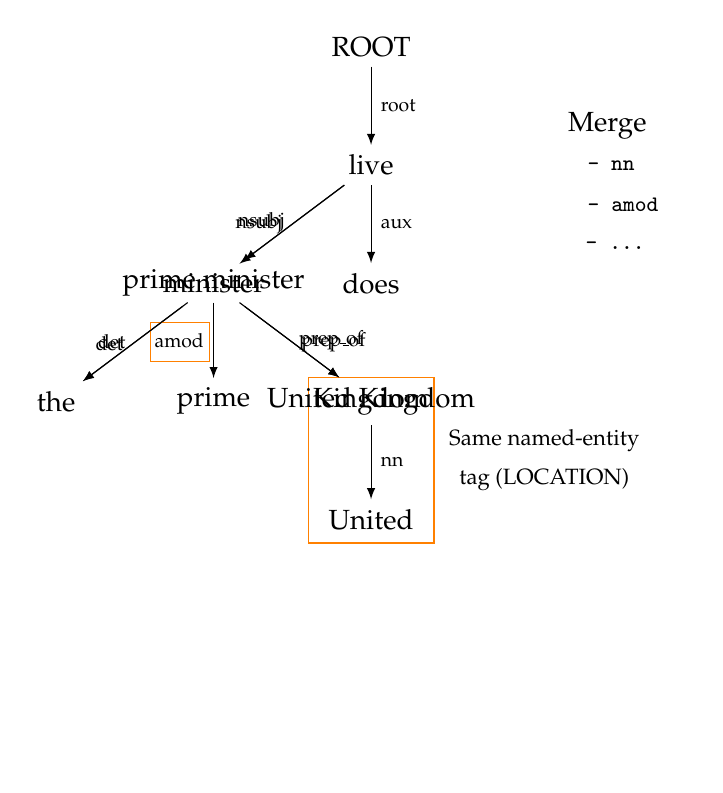
\begin{tikzpicture}
  \node (0) at (10,10) {ROOT};
  \node (1) at (10,8.5) {live};
  \onslide<-3>{\node (2) at (8,7) {minister};}
  \node (3) at (10,7) {does};
  \node (5) at (6,5.5) {the};
  \onslide<-3>{\node (6) at (8,5.5) {prime};}
  \onslide<1>{\node (7) at (10,5.5) {Kingdom};}
  \onslide<1>{\node (8) at (10,4) {United};}

  \node (9) at (14,1) {}; % utilisé pour forcer le positionnement de la figure globale

  \onslide<1>{\draw [draw=orange] (9.2,5.8) rectangle (10.8,3.7);}
  \onslide<1>{\node (10) at (12.2,5) {\footnotesize{Same named-entity}};}
  \onslide<1>{\node (11) at (12.2,4.5) {\footnotesize{tag (\alert{LOCATION})}};}

  \onslide<2->{\node (12) at (10,5.5) {United Kingdom};}

  \draw[->, >=latex] (0) edge node[anchor=center, right] {\scriptsize{root}} (1);
  \onslide<-3>{\draw[->, >=latex] (1) edge node[anchor=center, left] {\scriptsize{nsubj}} (2);}
  \draw[->, >=latex] (1) edge node[anchor=center, right] {\scriptsize{aux}} (3);
  \onslide<-3>{\draw[->, >=latex] (2) edge node[anchor=center, left] {\scriptsize{det}} (5);}
  \onslide<-3>{\draw[->, >=latex] (2) edge node[anchor=center, right] {\scriptsize{prep\_of}} (7);}
  \onslide<-3>{\draw[->, >=latex] (2) edge node[anchor=center, left] {\scriptsize{amod}} (6);}
  \onslide<1>{\draw[->, >=latex] (7) edge node[anchor=center, right] {\scriptsize{nn}} (8);}
  
  % fusion du amod
  
  \onslide<3>{\draw [draw=orange] (7.2,6.5) rectangle (7.95,6);}
  
  \onslide<3,4>{
  \node (13) at (13,9) {\alert{Merge}};
  \node (14) at (13.05,8.5) {\footnotesize{\texttt{- nn}}}; 
  \node (15) at (13.2,8) {\footnotesize{\texttt{- amod}}}; 
  \node (16) at (13.1,7.5) {\footnotesize{\texttt{- ...}}};}

  \onslide<4->{\node (17) at (8,7) {prime minister};}
  \onslide<4>{\draw[->, >=latex] (1) edge node[anchor=center, left] {\scriptsize{nsubj}} (17);}
  \onslide<4>{\draw[->, >=latex] (17) edge node[anchor=center, right] {\scriptsize{prep\_of}} (7);}
  \onslide<4>{\draw[->, >=latex] (17) edge node[anchor=center, left] {\scriptsize{det}} (5);}
  \end{tikzpicture}
\end{figure}
  
\end{frame}

%#############################################################################################################%
%#############################################################################################################%

\begin{frame}[fragile]
  \frametitle{Removal}

\begin{figure}
 \begin{tikzpicture}
  \node (0) at (10,10) {ROOT};
  \node (1) at (10,8.5) {live};
  \node (2) at (8,7) {prime minister};
  \onslide<1>{\node (3) at (10,7) {does};}
  \onslide<1>{\node (5) at (6,5.5) {the};}
  \node (7) at (10,5.5) {United Kingdom};

  \node (8) at (14,1) {}; % utilisé pour forcer le positionnement de la figure globale

  \onslide<1>{\draw [draw=orange] (6.4,6.5) rectangle (7,5.9);}
  \onslide<1>{\draw [draw=orange] (10.05,7.9) rectangle (10.6,7.6);}
  
  \node (9) at (13,9) {\alert{Remove}};
  \node (10) at (13.1,8.5) {\footnotesize{\texttt{- det}}}; 
  \node (11) at (13.1,8) {\footnotesize{\texttt{- aux}}}; 
  \node (12) at (13.1,7.5) {\footnotesize{\texttt{- ...}}};
  
  \draw[->, >=latex] (0) edge node[anchor=center, right] {\scriptsize{root}} (1);
  \draw[->, >=latex] (1) edge node[anchor=center, left] {\scriptsize{nsubj}} (2);
  \onslide<1>{\draw[->, >=latex] (1) edge node[anchor=center, right] {\scriptsize{aux}} (3);}
  \onslide<1>{\draw[->, >=latex] (2) edge node[anchor=center, left] {\scriptsize{det}} (5);}
  \draw[->, >=latex] (2) edge node[anchor=center, right] {\scriptsize{prep\_of}} (7);

  \onslide<2>{} % forcer slide 2
  \end{tikzpicture}
\end{figure}
  
\end{frame}


%#############################################################################################################%
%#############################################################################################################%

\begin{frame}[fragile]
  \frametitle{Nounification}

\begin{figure}
 \begin{tikzpicture}
  \node (0) at (10,10) {ROOT};
  \onslide<1>{\node (1) at (10,8.5) {live};}
  \node (2) at (8,7) {prime minister};
  \node (7) at (10,5.5) {United Kingdom};

  \node (8) at (6.45,1) {}; % utilisé pour forcer le positionnement de la figure globale

  \onslide<1>{\draw[->, >=latex] (0) edge node[anchor=center, right] {\scriptsize{root}} (1);}
  \onslide<1>{\draw[->, >=latex] (1) edge node[anchor=center, left] {\scriptsize{nsubj}} (2);}
  \draw[->, >=latex] (2) edge node[anchor=center, right] {\scriptsize{prep\_of}} (7);
  
  \node (18) at (12.7,9) {\alert{Nounify}};
  \onslide<1>{\draw [draw=orange] (9.6,8.7) rectangle (10.4,8.3);}
  
  \onslide<2->{\node (22) at (10,8.5) {residence};}
  \onslide<2->{\draw[->, >=latex] (0) edge node[anchor=center, right] {\scriptsize{root}} (22);}
  \onslide<2->{\draw[->, >=latex] (22) edge node[anchor=center, left] {\scriptsize{nsubj}} (2);}
  \end{tikzpicture}
\end{figure}
  
\end{frame}

%#############################################################################################################%
%#############################################################################################################%

\begin{frame}[fragile]
  \frametitle{Replacement rules}

\begin{figure}
 \begin{tikzpicture}
  \node (0) at (10,10) {ROOT};
  \node (22) at (10,8.5) {residence};
  \node (2) at (8,7) {prime minister};
  \node (7) at (10,5.5) {United Kingdom};

  \node (8) at (14,1) {}; % utilisé pour forcer le positionnement de la figure globale

  \onslide<1>{\draw[->, >=latex] (0) edge node[anchor=center, right] {\scriptsize{root}} (22);}
  \onslide<1>{\draw[->, >=latex] (22) edge node[anchor=center, left] {\scriptsize{nsubj}} (2);}
  \onslide<1>{\draw[->, >=latex] (2) edge node[anchor=center, right] {\scriptsize{prep\_of}} (7);} 
  
  \onslide<1>{\draw [draw=orange] (10.05,9.5) rectangle (10.7,9);}
  \onslide<1>{\draw [draw=orange] (8.2,8) rectangle (9,7.6);}
  \onslide<1>{\draw [draw=orange] (9,6.5) rectangle (10.1,6);}

  \node (18) at (12.7,9) {\alert{Replace}};
  \node (19) at (14.55,8.5) {\footnotesize{\texttt{- nsubj, prep\_of, ...} $\rightarrow R_5$}}; 
  \node (20) at (14.2,8) {\footnotesize{\texttt{- comp, vmod, ...} $\rightarrow R_3$}}; 
  \node (21) at (12.8,7.5) {\footnotesize{\texttt{- ...}}};

  \onslide<2->{\draw[->, >=latex] (0) edge node[anchor=center, right] {\scriptsize{$R_0$}} (22);}
  \onslide<2->{\draw[->, >=latex] (22) edge node[anchor=center, left] {\scriptsize{$R_5$}} (2);}
  \onslide<2->{\draw[->, >=latex] (2) edge node[anchor=center, right] {\scriptsize{$R_5$}} (7);}
  \end{tikzpicture}
\end{figure}
  
\end{frame}

%#############################################################################################################%
%#############################################################################################################%

\begin{frame}[fragile]
  \frametitle{Normalization}
  
\begin{figure}
 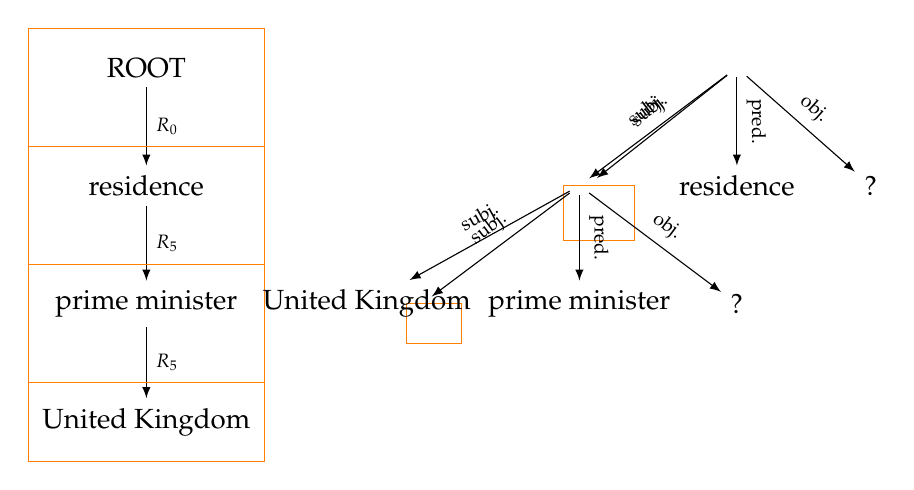
\begin{tikzpicture}
  \node (0) at (9,10) {ROOT};
  \node (1) at (9,8.5) {residence};
  \node (2) at (9,7) {prime minister};
  \node (3) at (9,5.5) {United Kingdom};

  \draw[->, >=latex] (0) edge node[anchor=center, right] {\scriptsize{$R_0$}} (1);
  \draw[->, >=latex] (1) edge node[anchor=center, right] {\scriptsize{$R_5$}} (2);
  \draw[->, >=latex] (2) edge node[anchor=center, right] {\scriptsize{$R_5$}} (3); 
  
  \onslide<1>{\draw [draw=orange] (7.5,10.5) rectangle (10.5,5);}
  \onslide<2>{\draw [draw=orange] (7.5,9) rectangle (10.5,5);}
  \onslide<3>{\draw [draw=orange] (7.5,7.5) rectangle (10.5,5);}
  \onslide<4>{\draw [draw=orange] (7.5,6) rectangle (10.5,5);}

  %%%%
  
  \onslide<3->{
  \node (4) at (16.5,10) {$\triple$};
  \node (5) at (14.6,8.5) {};
  \node (6) at (16.5,8.5) {residence};
  \node (7) at (18.2,8.5) {?};

  \draw[->, >=latex] (4) edge node[sloped, anchor=center, above] {\scriptsize{pred.}} (6);
  \draw[->, >=latex] (4) edge node[sloped, anchor=center, above] {\scriptsize{obj.}} (7); }
  \onslide<3>{\draw[->, >=latex] (4) edge node[sloped, anchor=center, above] {\scriptsize{subj.}} (5);}
  
  \onslide<3>{\draw [draw=orange] (14.3,8.5) rectangle (15.2,7.8);}

  \onslide<4->{
  \node (8) at (14.5,8.5) {$\triple$};
  \node (9) at (12.5,7) {};
  \node (10) at (14.5,7) {prime minister};
  \node (11) at (16.5,7) {?};

  \draw[->, >=latex] (4) edge node[sloped, anchor=center, above] {\scriptsize{subj.}} (8);
  \draw[->, >=latex] (8) edge node[sloped, anchor=center, above] {\scriptsize{pred.}} (10);
  \draw[->, >=latex] (8) edge node[sloped, anchor=center, above] {\scriptsize{obj.}} (11); }

  \onslide<4>{\draw[->, >=latex] (8) edge node[sloped, anchor=center, above] {\scriptsize{subj.}} (9);}

  \onslide<4>{\draw [draw=orange] (12.3,7) rectangle (13,6.5);}
  
  \onslide<5>{\node (12) at (11.8,7) {United Kingdom};
  \draw[->, >=latex] (8) edge node[sloped, anchor=center, above] {\scriptsize{subj.}} (12);}
 \end{tikzpicture}
\end{figure}

\end{frame}
    \label{reformulation}
    \section{Reformulation: a learning approach }
\label{mlreformulation}

\FloatBarrier

Efficiency of neural network nowadays can be very good. An approach based on network is also used here. But, the aim is not to learn answering question. There are two reasons for that. First the knowledge changes over time, e.g. the president name depends on the date. Then, something simple is wished. The learning process should also not be continuous. Learning the answer implies to know proper Names which increase the size of the dictionary, that means increasing the learning time. 

The module presented here tries to reformulate a question. In fact it tries to translate the question for the wikidata module. It means adapting it as most as possible for this module, correct the mistakes of grammatical parsing, as it is illustrated in figure \ref{figexmlrefref}.

\begin{figure}
    \centering
  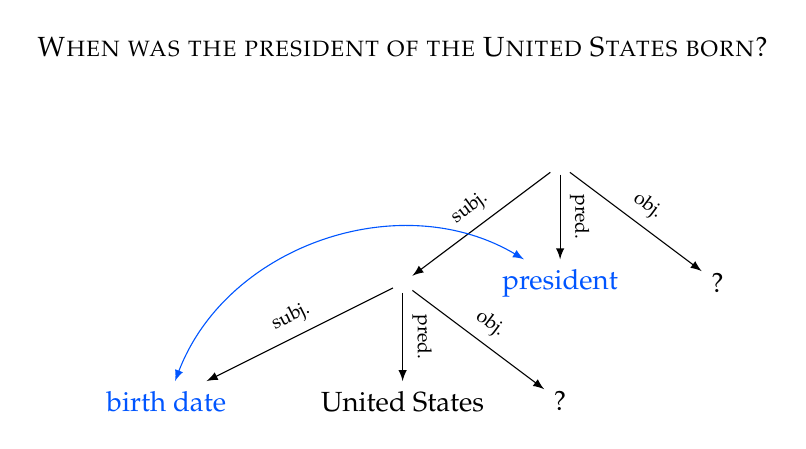
\begin{tikzpicture}
  \node (10) at (8,11.5) {\textsc{When was the president of the United States born?}};
  \node (0) at (10,10) {$\triple$};
  \node[color=mLightBrown] (1) at (10,8.5) {president};
  \node (2) at (12,8.5) {?};
  \node (3) at (8,8.5) {$\triple$};
  \node (4) at (8,7) {United States};
  \node[color=mLightBrown] (5) at (5,7) {birth date};
  \node (6) at (10,7) {?};

  \draw[->, >=latex] (0) edge node[sloped, anchor=center, above] {\scriptsize{pred.}} (1);
  \draw[->, >=latex] (0) edge node[sloped, anchor=center, above] {\scriptsize{obj.}} (2);
  \draw[->, >=latex] (0) edge node[sloped, anchor=center, above] {\scriptsize{subj.}} (3);
  \draw[->, >=latex] (3) edge node[sloped, anchor=center, above] {\scriptsize{subj.}} (5);
  \draw[->, >=latex] (3) edge node[sloped, anchor=center, above] {\scriptsize{obj.}} (6);
  \draw[->, >=latex] (3) edge node[sloped, anchor=center, above] {\scriptsize{pred.}} (4);
  \draw[<->, >= latex,color=mLightBrown] [draw=mLightBrown] [bend right=50, above] (1) edge (5);
  
 \end{tikzpicture}
 \caption{An example of bad triple formation, ``president'' and ``United States'' terms are in the wrong place. The reformulation module should solve this kind of problem.}
\label{figexmlrefref}
\end{figure}

\FloatBarrier
\subsection{How it works}


The grammatical module builds a tree representation of the question. The reformulation module work on this output, so with a tree representation. The assumption ``all useful information is kept in this form''  is also necessary. The module has also a dictionary. There are four steps to do. First a pretreatment replace proper names and numbers with tags, such that all words of the triple are in the dictionary, then the request is projected in the math space of request. Two last steps reveres the two first, but the reverse projection should produce a better request, which mean the final request is adapted for the Wikidata module.

For compatibilities reasons, we do not work with the actual data model which is too complicated. In fact we need a regular triple representation, that means all operators must be transformed, this step is easy. For unitary operators, $O(f)$ becomes $(f,O,?)$; for binary operators, $aOb$ becomes $(a,O,b)$. This operation does not weak the expressive power.

\subsubsection{Mathematical spaces}

The mathematical space of request $\mathcal{R}$ is simply the subset of the $\mathbb{R}$ vector space of dimension 50, were all vector have a Euclidean norm of 1.
A triple is formed of a subject request, a predicate and an object request, it is also natural to consider the triple over $\mathcal{R}$, which elements order with always be subject, predicate, object.
Let us call vector the elements of $\mathcal{R}$.

The choice of a 50-dimension can be modified if necessary, but taking a higher dimension could slow the learning process, and with a lower space we could lose some expressive power, which may lead to very poor results.

%To unify everything As we works with requests, we consider everything is a request, even a word.

%There are 2 generic spaces: the one of words which is a vector space of dimension 50 and the space of request which is the space of word triples. The first word of a triple represents the subject, the second represents the predicate and the last the object.
%To distinguish words which are vectors and words with letters, we will add the adjective English to the seconds.

\subsubsection{Dictionary}

The dictionary defines matching between English words and vectors triple, which is the base of the process. We use triple because a word could have different meaning depending on his nature, so predicate vector for a word is not the same as subject vector which is not the same as object vector. We will denote m.s subject vector of word m, m.p and m.o for predicate and object.

\subsubsection{Pre- and post-treatment and treatment}

We evoke some reasons not to handle proper name directly (the dictionary size would increase and names could change), there is another argument: there is an arbitrary number of proper names, because you can invent some new names every time. That is why they are replaced in a request by a tag NAMEi, $i\in{1,2,3}$. It allows us to have three different names in a question, and that is sufficient. The same happens to the numbers. Tag UNKNOWN finally represents the ``holes'' in the request tree. At the end, after the treatment we replace tags with corresponding real names or numbers in the final tree.

Recognizing a number is not hard, in fact it is just checking it the character sequence looks like numbers optionally followed by a dot and numbers. If the sequence is not a number or a ``hole'' and is not in the dictionary, the module treats it as a proper name.

\subsubsection{Project form a request to a vector}

The model allows an arbitrary request form, it means we have a tree with an unknown depth, and to keep the complete question information we should handle it so. But the request are triple, so it is easy to transform. First with the dictionary all words are replaced with vectors, of course we take the vector corresponding to the function of the word in the tree. Then we have to ascend the whole tree to compute the root value.

Let define a matrix compact which takes a triple of vector and merge them in one vector, here merging in not an intuitive operation, in fact we don't know how to merge this triple, that is why all coefficients of the matrix are unknown. To compute what we call a vector, output should be normalized.

Now by applying this operation bottom-up in the tree. The main idea is each node value represent the subtree request. A tree illustrates this on figure \ref{figexmlrefref}.

\FloatBarrier

\begin{figure}
\centering
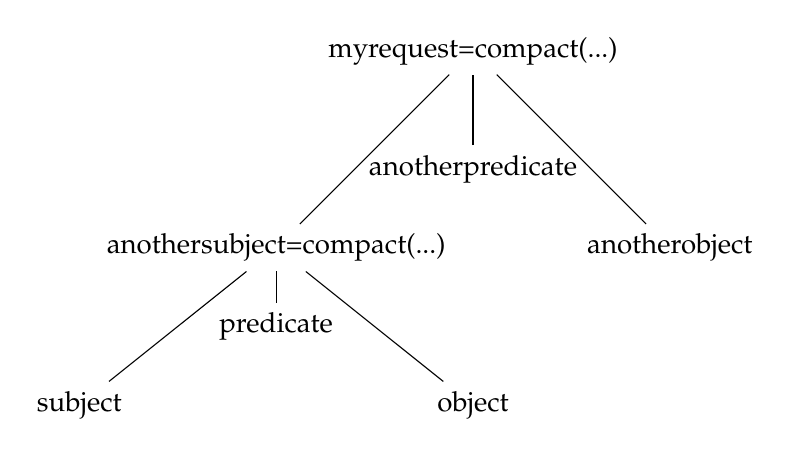
\begin{tikzpicture}[x=2.5cm]
\node (s) at (1,0) {subject};
\node (p) at (3,0) {object};
\node (r) at (2,1) {predicate};


\node (a) at (2,2) {anothersubject=compact(...)};
\node (b) at (4,2) {anotherobject};
\node (l) at (3,3) {anotherpredicate};
\node (h) at (3,4.5) {myrequest=compact(...)};

\draw (s)--(a)--(p);
\draw (r)--(a);
\draw (a)--(h)--(b);
\draw (l)--(h);
\end{tikzpicture}
\caption{The process of projection, an example}
\label{figexmlrefcomp}
\end{figure}

\FloatBarrier

\subsubsection{Reconstruct a request from a vector}

This operation is quite symmetrical of the projection, with a matrix uncompact we can the same way obtain a vector triple from a vector, and recursively a tree appear. But the question is how to know if we should reapply the function uncompact or leave the vector as a leaf? First say in a triple predicate is never a tree, then object and subject will be let as leaf if a known word is near enough. Finally each node is replaced with the nearest corresponding word in the dictionary, that mean, for example, for a vector in middle of a triple which is also a predicate, take word with nearest predicates' vector.

Defining near enough is difficult. To avoid infinite loop we will take depth of nodes into account. We must take $\delta>0$ a precision factor and $g$ a growth factor. If $d$ is the depth of node $n$, near enough means distance is bounded by $\delta*g^d$ with regard of Euclidean norm.  

\begin{figure}
\centering
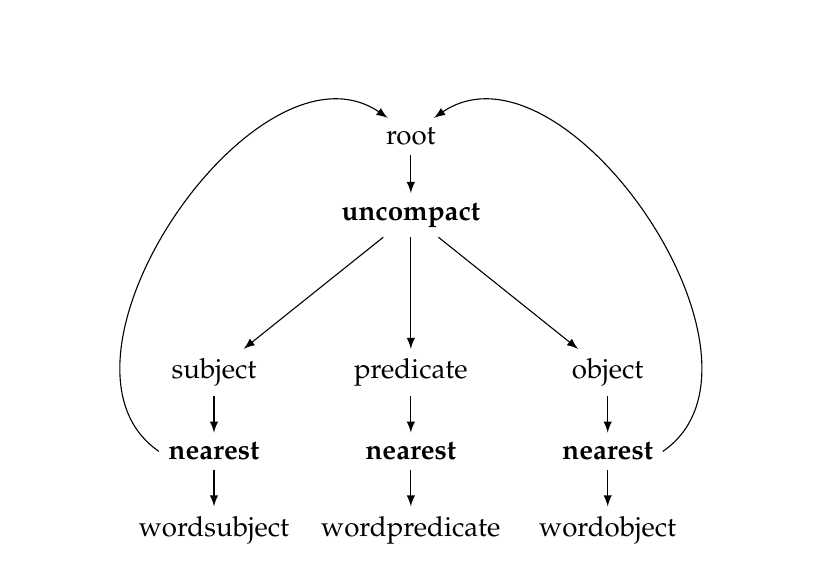
\begin{tikzpicture}[x=2.5cm]
\node (s) at (1,0) {subject};
\node (p) at (3,0) {object};
\node (r) at (2,0) {predicate};
\node (sf) at (1,-1) {\textbf{nearest}};
\node (pf) at (3,-1) {\textbf{nearest}};
\node (rf) at (2,-1) {\textbf{nearest}};
\node (sw) at (1,-2) {wordsubject};
\node (pw) at (3,-2) {wordobject};
\node (rw) at (2,-2) {wordpredicate};
\node[rectangle] (b) at (2,2) {\textbf{uncompact}};
\node (v) at (2,3) {root};
%\node (b) at (4,2) {b};
%\node (l) at (3,3) {l};
%\node (h) at (3,4) {h=compact(a,l,b)};

\draw[->, >=latex] (b)--(s);
\draw[->, >=latex] (b)--(p);
\draw[->, >=latex] (b)--(r);
\draw[->, >=latex] (v)--(b); % WTF?
\draw[->, >=latex] (r)--(rf);
\draw[->, >=latex] (p)--(pf);
\draw[->, >=latex] (s)--(sf);
\draw[->, >=latex] (rf)--(rw);
\draw[->, >=latex] (pf)--(pw);
\draw[->, >=latex] (sf)--(sw);

\draw [->, >=latex] (pf.east)        to [bend right=90] (v);
\draw [->, >=latex] (sf.west)        to [bend left=90] (v);
\end{tikzpicture}
\caption{The algorithm \textsc{reconstruction} in a scheme}
\label{figexmlrefunal}
\end{figure}

The algorithm reconstruct is also:



\begin{algorithm}[H]
    \DontPrintSemicolon  % Some LaTeX compilers require you to use \dontprintsemicolon instead
    \KwIn{$\delta>0$ and $a\in A$}
    \KwOut{request tree}
    $(s,p,o) \gets \text{uncompact}(a)$\;
    Find m s.t. $\N{m.s-s}<\delta$ is minimal \;
    \lIf{m exists}{
        $s \gets m$
    }
    \lElse{
        $s \gets reconstruct(\delta*g,s)$
    } 
    Find m s.t. $\N{m.o-o}<\delta$ is minimal \;
    \lIf{m exists}{
        $o \gets m$
    }
    \lElse{
        $o \gets reconstruct(\delta*g,o)$
    } 
    $p \gets {\text{argmin}}_m  (\N{m.p-p})$\;
    \Return{$(s,r,o)$}\;
    \caption{\textsc{reconstruct} From vector to tree}
\end{algorithm}

You can find a scheme version of the algorithm on figure \ref{figexmlrefunal}.

\FloatBarrier

\subsubsection{Remarks}

Matrix compact and uncompact are not bijective after restraining the request space to existent requests. Applying uncompact then compact should give the identity, with of course an error margin, but when compacting then uncompacting we only have to find an equivalent request, i.e. with the same meaning but with another formulation. If it were not the case it would produce exactly the same output as the input, that would be useless.

\subsection{Learning}

Training the model cannot be done easily with a classic back-propagation because we have no idea what is the best triple for a question. The solution is also to try to change a little the matrix, and see what changes improve the better the quality of result, it is however very bad in cost. 

Now to compute the quality of the result, i.e. the score  of the module we use a semantic distance: it's a norm depending on the meaning of words. To be simple we base it of the relation graph ``instance of'' of Wikidata assuming it is a directed acyclic graph. We compute the nearest common ancestor and we add the distance between this node and the two word  nodes.

\subsection{Implementation}

The module is written in C++, with threads to speed up the matrix multiplication. To interface it with the others, it is built as a shared library with python library. The dictionary has been generated using the clex \footnote{\url{https://github.com/Attempto/Clex}}. 

\subsection{Future work}

The learning process has not been made yet. As latency with Wikidata is very high (several seconds) we have to download Wikidata and run it in local.

Then we could think of different manners to train the model.

At least we could think about a good manner to find the nearest word in the dictionary. It can be done with a linear time, but considering there are 100 000 words in the dictionary, cost is not negligible. As we work in dimension 50, it is not a trivial problem to find an efficient method to obtain a logarithmic complexity. Kd-trees allow a search in log-time (with preprocessing); but with dimension 50, the constant factor $2^{50}$ is too large. One line of research were to use distance sensitive hash.

%Finding a way to learn everything with first or second approach is the most important, as the first answering module in functional, learning is possible. Then, learning and computation speed-up will be important, the search for nearest neighbor is long, maybe it is linear, but with near 100 000 words and high dimension it becomes consequent, use of heuristics could be a good idea, for example there exists distance sensitive hash.


    \label{standalone}
    \subsection{Machine Learning \--- Standalone}

\begin{frame}[fragile]
  \frametitle{Keywords questions}

	
	\begin{center}
  	\alert{United States president}
	\end{center}

	\begin{center}
  	\alert{president United States}
	\end{center}

\end{frame}

\begin{frame}[fragile]

Classify each word into one of the four categories: \{to ignore, subject, predicate, object \}

\end{frame}

\begin{frame}[fragile]

	\begin{center}
  	\alert{(United, subject) (States, subject) (president, predicate)}
	\end{center}

	\begin{center}
  	\alert{(president, predicate) (United, subject) (States, subject)}
	\end{center}



\end{frame}

\begin{frame}[fragile]
  \frametitle{Look-up table}

	\begin{center}
	Word $w \Rightarrow $ Vector $ V_w \in \mathbb{R}^{25}$
	\end{center}

	\begin{center}
	If two words $w_1$ and $w_2$ are synonymous then, \newline
	$$ || w_2 - w_1 ||_2 \approx 0 $$
	
	\end{center}



\end{frame}





\chapter{Wikidata module}
    \label{wikidata}
    \section{Wikidata}

\subsection{Overview}
Wikidata module\footnote{\url{https://github.com/ProjetPP/PPP-Wikidata/}} is our main proof of concept module which aims to demonstrate the ability of our framework to allow the easy creation of huge modules able to answer thousand of questions. This module tries to answer general knowledge using the data stored in Wikidata\footnote{\url{http://www.wikidata.org/}}.

\begin{figure}[!ht]
  \centering
    \label{wikidata:item-screenshot}
    \includegraphics[width=\textwidth]{./wikidata-item-screenshot.png}
    \caption{The beginning of a Wikidata item}
\end{figure}

Wikidata is a free knowledge base hosted by the Wikimedia Foundation as a sister project of Wikipedia. It aims to build a free, collaborative, multilingual structured database of general knowledge (for more information see \cite{42240}). It provides a very good set of API that allows to consume and query Wikidata content easily. Wikidata is built upon entities (called items and stored in a separated wiki pages) that are about a given subject. Each item has a label, a description and some aliases to describe it and statements that provides data about this subject (see figure \ref{wikidata:item-screenshot}). Each statement is built around a property and a value such that $(item, property, value)$ may be seen as a valid triple. Properties are entities like items and so may have labels, descriptions, aliases and statements. For more information see\footnote{\url{http://www.wikidata.org/wiki/Wikidata:Glossary}}.

We have chosen Wikidata instead of some other famous knowledge base like DBpedia\footnote{\url{http://dbpedia.org}} or Freebase\footnote{\url{http://www.freebase.com/}} because Wikidata is under a CC0 license\footnote{\url{http://creativecommons.org/publicdomain/zero/1.0/}} that allows to reuse data without constraints and is fully multilingual, a characteristic that will be very useful in order to adapt the PPP to other languages than English. More, as one of the members of the team is involved in Wikidata it allows us to avoid to lose time by learning the other knowledge base APIs.

\subsection{APIs}
Wikidata provides an API that allows to retrieve items and properties from there ids and an API that returns items or properties that match a given label. For more information about the API see the appendix \ref{wikidata:api-examples}.

Some libraries are available to interact easily with the API. The two major ones are:
\begin{itemize}
    \item \textbf{Wikidata Toolkit}\footnote{\url{http://www.mediawiki.org/wiki/Wikidata_Toolkit}} written in Java and allows to interact easily with the API and dumps of Wikidata content that are regularly done.
    \item \textbf{wikibase-api}\footnote{\url{https://github.com/addwiki/wikibase-api}} written in PHP that only allows to interact with the API but has the strong advantages to share a lot of code with the MediaWiki extension that powers Wikidata\footnote{\url{https://www.mediawiki.org/wiki/Wikibase}}.
\end{itemize}

We have chosen to use the PHP API because one of the members of the team has contributed in a significant manner to it and so was able to have a working module quickly.

In order to do queries in Wikidata content, like retrieving all presidents of the United States, e.g. all items with the property "position held" (P39) with value "president of the united States of America" (Q11696) we had to rely on an external service, called \textbf{WikidataQuery}\footnote{\url{http://wdq.wmflabs.org/}} that allows to do such requests. This was needed because the Wikidata API does not allow to do such queries yet. We have written a small standalone and reusable wrapper to the API of this service in PHP\footnote{\url{https://github.com/ProjetPP/WikidataQueryApi/}}.

\subsection{Implementation}
In order to write this module nicely we have written a small PHP library, LibModule\url{https://github.com/ProjetPP/PPP-LibModule-PHP}, that provides a framework to create PPP modules and diverse utilities to simplify nodes like union or intersection that do not requires specific knowledge about the resources themselves.

This module works in tree steps:
\begin{enumerate}
    \item It maps \textit{resource} nodes of the question tree into Wikidata content: the subjects of \textit{triple} nodes are mapped to Wikidata items, predicates to Wikidata properties and objects to the type of value that is the range of the Wikidata property of the predicate. If more than one match are possible, a tree per possible match is output.
    \item It performs queries against Wikidata content using the previously done mapping to reduce as much as possible trees. When we have a \textit{triple} node where the object is missing the module gets the Wikidata item of the subject, looks for values for the predicate property and replace the \textit{triple} node with a \textit{resource} node for each value of the triple (and so builds as many trees as there are values). When there is a \textit{triple} node with a missing subject the module uses the WikidataQuery API.
    \item It adds clean representation of \textit{resource} nodes added by the previous phase. When Wikidata resources are returns it keeps their IDs in order to allow the ui to create nice display of them.
\end{enumerate}

We have also added specific support for "name", "definition" and "identity" predicates in order to allows the API to have a nice display of the "Barack Obama" item when the query is "Who is Barack Obama?", rewritten as \textit{(Barack Obama, identity, ?)}. the same thing applies if the module input is a sentence like "Barack Obama".

One of the difficulties met was to avoid meaningless results because Wikidata contains items about Wikipedia organizational content like "disambiguation" or "category" pages. So we have written a small filter that ignore these pages when the conversion string to Wikidata identifier is done.

\begin{figure}[!h]
  \centering
    \label{wikidata:struct}
    \includegraphics[width=\textwidth]{./wikidata_louis13_children.png}
    \caption{An example output from the Wikidata module}
\end{figure}

\subsection{Future work}

This module is only at its first stage and a lot of nice to have features remains:
\begin{itemize}
    \item Clever filter of not relevant results: people that are looking for the list of the presidents of the United States are usually not looking for fictional ones.
    \item Handle triple that does not directly match to Wikidata model. If we looks for people born in France we are also looking for people born in Lyon or if we are looking for the American Secretary of State we are looking for the person that has as office "American Secretary of State".
    \item Do some reasoning on Wikidata content. For example if \texttt{(Lyon, instance of, city)} and \texttt{(city, subclass of, place)} then we should be able to guess and use that \texttt{(Lyon, instance of, place)}.
\end{itemize}

    
\chapter{CAS module}
    \label{cas}
    \newcommand{\CalChAS}{\text{C}\hspace{-2pt}_{\text{AL}}\hspace{-3pt}\text{C}^{\text{H}}{\hspace{-4pt}}_\text{AS}}
\newcommand{\RR}{\mathbb{R}}
\newcommand{\CC}{\mathbb{C}}
\newcommand{\ZZ}{\mathbb{Z}}
\newcommand{\NN}{\mathbb{N}}
\newcommand{\dd}{\mathrm{d}}


A computer algebra system (CAS) module has been added to the PPP. Its work is to compute formally mathematical expressions.

\section{Input-output}

The CAS module take as input a sentence whose string is a mathematical expression and output a resource of typed \texttt{math-latex} with two fields: one with a human readable formula and the other written in \LaTeX.

The difficulty is two decide whether a string represent a mathematical formula or not.

We use two tests. The first is a pre-treatment test. It checks whether the formula contains some substring which prove
\begin{itemize}
    \item the formula is a mathematical expression, like "sqrt", "\textbackslash"\ldots,
    \item the formula is not a mathematical expression, like "who", "where", accented character\ldots.
\end{itemize}

But that does not eliminate all natural language questions, there still are false positive. Nevertheless, this test is basic and works in the larger part of cases.

\bigskip

So there is another test which is more precise. For example, a query like "author of bli-bla" will not be excluded by the previous algorithm. Moreover we see here why we can't consider '-' as a characteristic character of mathematical formula. The method is to verify if the module apply modifications.

Is this example, the module has nothing to compute and car just rearrange terms. So "author of bli-bla" become something like "author bli of - bla" considering 'author', 'bli', 'bla' and 'of' as variable. But we observe there was no modification. To do this test, the module counts each kind of symbol (except space and some particular symbols). If there is the same quantity of each symbol, we consider there is no modifications and the module decides he was useless and returns an empty list.

\section{Structure}

To do mathematical computations, we use a specific library: Sympy\footnote{\url{http://www.sympy.org/en/index.html}}. But this library is able to analyse only the input write with the good syntax which is not intuitive and pretty complex.

To avoid arbitrary long computation, we launch Sympy evaluation in another process which has a limited memory and time.

To be usable, we define two parsers to handle other syntax: the syntax of Mathematica and another syntax we defined, which is designed to be intuitive and we named $\CalChAS$.

\section{Parsers}

\subsection{Mathematica parser}

This parser is quite simple. We use a LALR parser generated by PLY\footnote{\url{http://www.dabeaz.com/ply/}} (Python Lex Yacc). First, the input formula is parsed and transform into a tree, then, the tree is transform into a Sympy expression.

\subsection{\texorpdfstring{$\CalChAS$}{CalChAS} parser}

This syntax is more permissive. It allows arithmetic operations (division, multiplication, addition, subtraction, modulo, factorial, power) and several names for each standard function. For instance, the 
reciprocal of the hyperbolic sine can be written "argsh", "argsinh", "arcsh" etc.. So function names are matched with regular expression. For instance, the regex for the function argsinh is \begin{center}[\texttt{aA}](\texttt{r}([cg])?)?[\texttt{sS}](\texttt{in})?\texttt{h}\end{center}

The other feature we implement for flexibility is implicit multiplications. We understand "a b" as "a*b", "(a)b" as "(a)*b" and "(a)(b)" as "(a)*(b)". But "a(b)" have to remain unchanged because "a" can be a function so, "a(b)" is not "a*(b)".

This transformation is executed before the parser. The method is to launch the lexer a first time. Then we add the symbol "*" between the two symbols in every followed configurations: ")("; a ")" and a identifier; two consecutive identifiers. Thus, we generate a modified formula with explicit multiplications and we can parse this expression.

The last feature implemented to make this syntax more permissive is to extend functions which are defined on a subset of $\RR$ like $\NN$. For example, the factorial which is defined on $\NN^*$ is extended on $\CC\setminus \ZZ^{-*}$ by using the function $\Gamma$. Thus, the expression $(-1/2)!$ has a meaning.

This syntax admits notation as defined in the standard ISO 31-11.

\section{Future work}

A parser for \LaTeX expressions can be implemented. We started to write a \LaTeX parser but it was more complicated than expected and actually, it does not work for big operators like sum, product or integral.

We can also cover other mathematical fields. For instance:
\begin{itemize}
    \item probability,
    \item statistics,
    \item regression analysis,
    \item logic and set theory,
    \item discrete mathematics,
    \item sequences,
    \item plots.
\end{itemize}

We can imagine a more lenient syntax for functions which need to bound a variable when there is no ambiguities. For instance, we plan to allow "int(sin(x),0,Pi)" for "int(sin(x),x,0,Pi)" because $x$ is the only variable in this expression. If we are able to determine the list of variables, there is easy to create a new variable. That allows to define functions like $(k,n)\mapsto \binom{n}{k}$ on a larger set using a limit.

An important missing feature is the resolution of differential equations. In fact the \texttt{dsolve} function of Sympy does not work on every ODE and does not handle initial conditions. If this feature is not implemented soon, we will use the \texttt{dsolve} function of Sympy without initial conditions and determine constants with the function \texttt{solve}.

The other feature to implement, is the interpretation of mathematical queries expressed in natural language. For example, "integrate sin x dx from x=0 to pi" instead of "integrate(sin(x),x,0,pi)".

\chapter{Spell checker}
    \label{spellchecker}
    \section{Spell Checker}

The spell checker is a Python module\footnote{\url{https://github.com/ProjetPP/PPP-Spell-Checker}}
which aims at correcting spelling mistakes in the sentence.
Indeed, errors are often made by the user, and we want to avoid her/his query to fail.

This module uses the \emph{GNU Aspell} library\footnote{\url{http://aspell.net/}},
with a Python wrapper\footnote{\url{https://github.com/WojciechMula/aspell-python}}.
Aspell is an open source software, and is the standard spell checker on GNU/Linux.

Here are the steps of the algorithm.

Input sentence:
\begin{center}
Who is the auhtor of "Le Petit Prince"?
\end{center}

Get all the words of the sentence:
\begin{center}
[Who, is, the, auhtor, of, Le, Petit, Prince]
\end{center}

Apply the Aspell corrector on each individual word which is not contained on a
quotation in the original sentence:
\begin{center}
[Who, is, the, author, of, Le, Petit, Prince]
\end{center}

Replace the words in the sentence, taking care of keeping the punctuation as is:
\begin{center}
Who is the author of "Le Petit Prince"?
\end{center}

Remark that it is necessary to keep the words of a quotation unchanged, otherwise
we would have modified "Le Petit Prince" since it is not correct English, although
it is the correct title of the book.


\chapter{OEIS module}
    \section{OEIS module}

The OEIS, Online Encyclopedia of Integer Sequences\footnote{\url{https://oeis.org/}}, is a database of integer
sequences; it contains their first numbers, name, description, etc.

This module\footnote{\url{https://github.com/ProjetPP/PPP-OEIS}} allows the
PPP to query this database in order to answer simple questions, like
“What follows 1, 2, 4, 8, 16, 32?”, or “What is 1, 2, 4, 8, 16, 32?”,
by using a small OEIS library\footnote{\url{https://github.com/ProgVal/Supybot-plugins/blob/master/OEIS/oeis.py}}
a member of the project wrote last year


\chapter{Performances}
    \label{performances}
    \section{Overview}

Our search engine, \emph{Platypus}, is able to answer correctly to a wide range
of questions.

Here is a non-exhaustive list of questions with correct answer.

\subsection{Keyword questions}

\begin{itemize}
    \item Definition question.
    \begin{verbatim}
    Sherlock Holmes
    \end{verbatim}

    \item Depth-1 question.
    \begin{verbatim}
    author Les Misérables
    \end{verbatim}
\end{itemize}

\subsection{English questions}

\begin{itemize}
    \item Definition question.
    \begin{verbatim}
    What is “P=NP”?
    \end{verbatim}

    \item Location question.
    \begin{verbatim}
    Where is the capital of New Zealand?
    \end{verbatim}

    \item Depth-1 question, with quotation marks.
    \begin{verbatim}
    Who is the author of “Le Petit Prince”?
    \end{verbatim}
\end{itemize}

\subsection{Math questions}

\begin{itemize}
    \item Approximation of $\pi$ to the $42^{th}$ digit.
    \begin{verbatim}
    N[Pi, 42]
    \end{verbatim}

    \item Exact value of $\lim_{n\rightarrow \infty} \sum_{i=1}^n \frac{1}{i} - \log(n)$.
    \begin{verbatim}
    Limit[Sum[1/i, {i,1,n}]-Log[n], n->Infinity]
    \end{verbatim}
\end{itemize}

\subsection{Weird questions}

\begin{itemize}
    \item Spelling mistake.
    \begin{verbatim}
    What is the cappyttal of Franse?
    \end{verbatim}

    \item Nested question.
    \begin{verbatim}
    Who are the daughters of the wife of the husband of the wife of the president
    of the United States?
    \end{verbatim}
\end{itemize}

\section{Comparison with existing tools}

We study the ability of our tool to successfully answer to questions, in comparison
to \emph{WolframAlpha}\footnote{\url{https://www.wolframalpha.com/}}, one of the best
question answering engine.

\subsection{Nested questions}

A nested question is a question with several level of knowledge. For instance, the
question "What is the birth date of the first person to walk on the moon?" requires
firstly to know that Neil \textsc{Armstrong} was the first person to walk on the
moon and then to know that he was born on August 5, 1930.

Our search engine tends to be more successful than \emph{WolframAlpha}
on such questions. We explain this by the fact that nested questions are generally
well structured and therefore good candidates for a grammatical analysis.

Some examples:

\begin{tabular}{l|l}
    \multicolumn{2}{l}{Who is the mayor of the capital of Czech Republic?} \\
    \hline
    \textbf{WolframAlpha} & Prague\\
    \textbf{Platypus} & Tomáš Hudeček\\
\end{tabular}

\begin{tabular}{l|l}
    \multicolumn{2}{l}{When was born the author of "Sherlock Holmes"?} \\
    \hline
    \textbf{WolframAlpha} & no result\\
    \textbf{Platypus} & Sunday, May 22, 1859\\
\end{tabular}

\begin{tabular}{l|l}
    \multicolumn{2}{l}{What is the citizenship of the daughters of the wife of the president of the United States?} \\
    \hline
    \textbf{WolframAlpha} & Barack Obama\\
    \textbf{Platypus} & United States of America\\
\end{tabular}

\subsection{Conjunction questions}

A conjunction is a question which require to do either an union of sets or an intersection
of sets. For instance, the question "Who has been a Jedi and a Sith?" requires to
compute the intersection of the members of the Jedi organization and the Sith organization,
to find out all the persons that has been in both organizations.

Thank to the union and the intersection of our data model, our search engine also
provide better answers for such questions.

An example:

\begin{tabular}{l|l}
    \multicolumn{2}{l}{Who is the actress of "Pulp Fiction" and "Kill Bill"?} \\
    \hline
    \textbf{WolframAlpha} & the whole casting of this two films\\
    \textbf{Platypus} & Uma Thurman\\
\end{tabular}


\section{Limitations}

Platypus is still limited to the knowledge of \emph{Wikidata} and to some grammatical
structures.

\emph{Wikidata} does not contain any information about measures. We are unable
to answer to questions like "How far is the Sun?", "How small is an atom?" or
"What is the speed of Ariane 5?".

We are also unable to parse correctly sentences with a more complex structure, like
"From which country does the jazz come from?".


\addcontentsline{toc}{chapter}{Conclusion}
\chapter*{Conclusion}
    \label{conclusion}
    \subsection{Better than Wolfram?}

\begin{frame}
    \frametitle{Nested question}

Who is the wife of the president of the United States?
    \begin{tabular}{ll}
        \alert{WolframAlpha} & Barack Obama\\
        \alert{Platypus} & Michelle Obama\\
    \end{tabular}

    \medbreak

    \onslide<2->{
        What are the birth dates of the daughters of the wife of the president of the United States?
        \begin{tabular}{ll}
            \alert{WolframAlpha} & Barack Obama\\
            \alert{Platypus} & Saturday, July 4, 1998 \& Sunday, June 10, 2001\\
        \end{tabular}
    }
\end{frame}

\begin{frame}[fragile]
    \frametitle{Conjunction}

Who is the actor of Inception and Titanic?
    \begin{tabular}{ll}
        \alert{WolframAlpha} & all the actors of the two movies\\
        \alert{Platypus} & Leonardo DiCaprio\\
    \end{tabular}
\end{frame}

\subsection{Future work}

\begin{frame}
    \frametitle{Better database}

    ``How fast is the TGV?''

    ``How wide is a tennis court?''

    Not answered by \alert{Wikidata}.

    \medbreak

    $\rightarrow$ Improve Wikidata?

    $\rightarrow$ Use another database?
\end{frame}

\begin{frame}
    \frametitle{Better question parsing}

    ``What is the date of birth of Isaac Newton?''

    ``In which band does Bono sing?''

    Not parsed correctly.

    \medbreak

    $\rightarrow$ Train the Stanford CoreNLP library?

    $\rightarrow$ Improve the algorithm of the Grammatical module?

    $\rightarrow$ Better datasets for the ML modules?
\end{frame}

\begin{frame}
    \frametitle{New modules}
\begin{figure}
 \begin{tikzpicture}
  \node (0) at (-3,2) {\textcolor{mLightBrown}{cooking recipes}};
  \node (0) at (1,1) {\textcolor{mDarkBrown}{HAL}};
  \node (0) at (5,2.5) {\textcolor{mMediumBrown}{meteo}};
  \node (0) at (3,2) {\textcolor{mDarkTeal}{chemistry}};
  \node (0) at (0,0) {\textcolor{mMediumBrown}{programming language interpreter}};
  \node (0) at (-4,-1) {\textcolor{mMediumBrown}{cinema}};
  \node (0) at (0,-2) {\textcolor{mDarkTeal}{music}};
  \node (0) at (4,-1) {\textcolor{mDarkTeal}{literature}};
  \node (0) at (-3,-2) {\textcolor{mDarkBrown}{OEIS}};
  \node (0) at (2,-2.5) {\textcolor{mLightBrown}{translation}};
  \node (0) at (-2,-3) {\textcolor{mMediumBrown}{sport statistics and predictions}};
  \end{tikzpicture}
\end{figure}
\end{frame}

\begin{frame}
    \frametitle{Other ideas...}

    \begin{itemize}
        \item Other languages support (French...)
        \item Improve user experience
        \item Advertise \alert{Platypus}
    \end{itemize}
\end{frame}

\subsection{Conclusion}

\begin{frame}
    \frametitle{Some facts} % to update just before the presentation
    \alert{23 repositories}

    \begin{tabular}{lll}
        6 & PHP & Wikidata libraries and module\\
        12 & Python & Other modules, core, and libraries\\
        1 & C++ & ML-Reformulation\\
        1 & Shell & Deployment scripts\\
        1 & \LaTeX & This presentation and the report\\
        1 & Markdown & The specification\\
        1 & HTML/CSS/Javascript & The Web User Interface\\
        1 & HTML/CSS & The project's website\\
    \end{tabular}

    \alert{1982 commits} (without the ``integration'' repository, which has an automatic commit every 12h)

    \alert{26k lines} of code (13k in PHP, 10k in Python)
\end{frame}

\begin{frame}
    \frametitle{The PPP?}

    \begin{itemize}
        \item A powerful question answering framework
        \item Innovative NLP algorithms
        \item A demo, \alert{Platypus}, with general knowledge and math
    \end{itemize}
\end{frame}


\newlength{\logosize}
\setlength{\logosize}{12pt}
\begin{frame}
    \frametitle{The adventure is only starting...}
    \alert{\url{http://projetpp.github.io/}}

    \begin{tabular}{ll}
        \includegraphics[width=\logosize]{Twitter_logo_blue.png} & \href{https://twitter.com/ProjetPP}{https://twitter.com/ProjetPP}\\
        \includegraphics[width=\logosize]{GitHub-Mark-32px.png} &  \href{https://github.com/ProjetPP}{https://github.com/ProjetPP}\\
        \includegraphics[width=\logosize]{ic_email_black_18dp.png} & \href{mailto:ppp@pony.ovh}{ppp@pony.ovh}\\
    \end{tabular}
\end{frame}


\begin{frame}
    \frametitle{Questions?}
    \begin{center}
        \includegraphics[height=0.7\textheight]{figures/Ornithorhynchus.jpg}
    \end{center}
\end{frame}

\begin{frame}
    \tikzset{
        workpackage/.style={
               node distance = 0.5cm,
               },
    }
    \frametitle{WorkPackages}
    \begin{figure}
        \begin{tikzpicture}
            % PPP members
            \node (rc)                  {Raphaël \textsc{Charrondière}};
            \node (qc)  [below of = rc] {Quentin \textsc{Cormier}};
            \node (tc)  [below of = qc] {Tom \textsc{Cornebize}};
            \node (yh)  [below of = tc] {Yassine \textsc{Hamoudi}};
            \node (mc)  [below of = yh] {Marc \textsc{Chevalier}};
            \node (vl)  [below of = mc] {Valentin \textsc{Lorentz}};
            \node (tpt) [below of = vl] {Thomas \textsc{Pellissier} \textsc{Tanon}};

            % PPP WorkPackages
            \node (reformulation)   [workpackage, right of = rc, right=3cm]  {Reformulation};
            \node (standalone)      [workpackage, below of = reformulation]  {Standalone};
            \node (spellchecker)    [workpackage, below of = standalone]     {SpellChecker};
            \node (communication)   [workpackage, below of = spellchecker]   {Communication};
            \node (grammatical)     [workpackage, below of = communication]  {Grammatical};
            \node (bibliography)    [workpackage, below of = grammatical]    {Bibliography};
            \node (cas)             [workpackage, below of = bibliography]   {CAS};
            \node (datamodel)       [workpackage, below of = cas]            {DataModel};
            \node (architecture)    [workpackage, below of = datamodel]      {Architecture};
            \node (core)            [workpackage, below of = architecture]   {Core};
            \node (sysadmin)        [workpackage, below of = core]           {System Administration};
            \node (wikidata)        [workpackage, below of = sysadmin]       {Wikidata};
            \node (webui)           [workpackage, below of = wikidata]       {WebUI};

            % Edges
            \path (reformulation.west)   edge (rc.east)
                  (standalone.west)      edge (qc.east)
                  (spellchecker.west)    edge (tc.east)
                  (communication.west)   edge (tc.east)
                  (grammatical.west)     edge (tc.east)
                  (grammatical.west)     edge (yh.east)
                  (bibliography.west)    edge (yh.east)
                  (datamodel.west)       edge (yh.east)
                  (datamodel.west)       edge (mc.east)
                  (datamodel.west)       edge (vl.east)
                  (datamodel.west)       edge (tpt.east)
                  (architecture.west)    edge (mc.east)
                  (architecture.west)    edge (vl.east)
                  (architecture.west)    edge (tpt.east)
                  (cas.west)             edge (mc.east)
                  (core.west)            edge (vl.east)
                  (sysadmin.west)        edge (vl.east)
                  (wikidata.west)        edge (vl.east)
                  (wikidata.west)        edge (tpt.east)
                  (webui.west)           edge (tpt.east);
        \end{tikzpicture}
    \end{figure}
\end{frame}


\bibliographystyle{alpha}
\bibliography{bibliography}
\nocite{*}

\appendix

\chapter{Question parsing \--- Triples tree}

\begin{figure}[!ht]
\begin{verbatim}
{
    "type": "triple",
    "subject": {
        "type": "triple",
        "subject": {
            "type": "resource",
            "value": "United States"
        },
        "object": {
            "type": "missing"
        },
        "predicate": {
            "type": "resource",
            "value": "president"
        }
    },
    "object": {
        "type": "missing"
    },
    "predicate": {
        "type": "resource",
        "value": "birth place"
    }
}

\end{verbatim}

\caption{Triples tree produced by the question parsing grammatical module on \textit{Where was the president of the United States born?}}
\label{triple_tree}
\end{figure}

\chapter{Question parsing \--- Grammatical rules analysis}

\begin{figure}[!ht]
\begin{footnotesize}
\begin{verbatim}
    undef     : R0
    root      : R0
    dep       : R1
        aux       : remove
            auxpass   : remove
            cop       : impossible
        arg       : impossible
            agent     : R5
            comp      : R3
                acomp     : R3
                ccomp     : R5
                xcomp     : R3
                pcomp     : R3
                obj       : impossible
                    dobj      : R5
                    iobj      : R3
                    pobj      : R3
            subj      : impossible
                nsubj     : R2 (if the output node is a leaf) 
                            R5 otherwise
                    nsubjpass    : R5
                csubj     : impossible
                    csubjpass    : impossible
        cc        : impossible
        conj      : apply global transformation (conjunction) and produce Rconj
        expl      : remove
        mod       : R4
            amod      : merge (if the tag of the output node is neither ORDINAL nor JJS) 
                        otherwise apply global transformation and produce Rspl
            appos     : R4
            advcl     : R4
            det       : remove
            predet    : remove
            preconj   : remove
            vmod      : R3
            mwe       : merge
                mark      : remove
            advmod    : merge
                neg       : apply global transformation (conjunction) and produce Rconj
            rcmod     : R4
                quantmod  : remove
            nn        : merge
            npadvmod  : merge
                tmod      : R3
            num       : merge
            number    : merge
            prep      : R5
            prepc     : R5
            poss      : R5
            possessive: impossible
            prt       : merge
        parataxis : remove
        punct     : impossible
        ref       : impossible
        sdep      : impossible
            xsubj     : R3
        goeswith  : merge
        discourse : remove
\end{verbatim}
\end{footnotesize}
\caption{Replacement rules used by the question parsing grammatical module (\texttt{impossible} means that the relation is not supposed to happen, or is not supported yet by our algorithm)}
\label{gramm_rule}
\end{figure}

\chapter{Wikidata API examples}
\label{wikidata:api-examples}
\section{Retrieve entities}

Goal: get the item \texttt{Q42} (Douglas Adams).

Request: \url{http://www.wikidata.org/w/api.php?action=wbgetentities&ids=Q42&format=json&languages=en}

Partial response:
\begin{lstlisting}[language=json]
{
    "entities": {
        "Q42": {
            "id": "Q42",
            "type": "item",
            "aliases": {
                "en": [{"language": "en", "value": "Douglas Noel Adams"}]
            },
            "labels": {
                "en": {"language": "en",  "value": "Douglas Adams"}
            },
            "descriptions": {
                "en": {"language": "en", "value": "English writer and humorist"}
            },
            "claims": {
                "P31": [
                    {
                        "id": "Q42$F078E5B3-F9A8-480E-B7AC-D97778CBBEF9",
                        "mainsnak": {
                            "snaktype": "value",
                            "property": "P31",
                            "datatype": "wikibase-item",
                            "datavalue": {
                                "value": "Q5",
                                "type": "wikibase-entityid"
                            }
                        },
                        "type": "statement"
                    }
                ]
            },
            "sitelinks": {
                "enwiki": {"site": "enwiki", "title": "Douglas Adams"}
            }
        }
    }
}
\end{lstlisting}


\section{Retrieve entities}

Gloal: get items for the label "Douglas Adams".

Request: \url{http://www.wikidata.org/w/api.php?action=wbgetentities&ids=Q42&format=json&languages=en}

Partial response:
\begin{lstlisting}[language=json]
{
    "searchinfo":{"search": "Douglas Adams"},
    "search":[
        {
            "id": "Q42",
            "url": "//www.wikidata.org/wiki/Q42",
            "description": "English writer and humorist",
            "label": "Douglas Adams"
        }
    ]
}
\end{lstlisting}


\section{Do search with WikidataQuery}

Gloal: get items that have "position held" (P39) "president of the united States of America" (Q11696).

Documentation: \url{http://wdq.wmflabs.org/api_documentation.html}

Request: \url{http://wdq.wmflabs.org/api?q=CLAIM[39:11696]}

Partial response:
\begin{lstlisting}[language=json]
{
    "items": [23, 76, 91, 207]
}
\end{lstlisting}

\chapter{CAS \--- \texorpdfstring{$\CalChAS$}{CalChAS} functions}
    We give here the functions and constants known by $\CalChAS$. As previously, we give regex in some cases. All variable name, function identifier or constant have to match [a-zA-Z\_][a-zA-Z0-9\_]*.

\section{Infix operators}
\begin{longtable}{ll}
    \caption[List of handled infix operators]{List of handled infix operators}\\
    \textbf{Regex} & \textbf{Operator} \\ 
    \endfirsthead

    \multicolumn{2}{c}
    {{\tablename\ \thetable{} -- List of handled infix operators}} \\
    \textbf{Regex} & \textbf{Operator} \\ 
    \endhead

    \multicolumn{2}{r}{{\--- Continued on next page \---}} \\ \endfoot

    \endlastfoot
    + & Addition \\
    - & Subtraction \\
    * & Multiplication \\
    / & Division \\
    \% & Modulo \\
    (\^{}|**) & Power \\
    ! & Factorial 
\end{longtable}

\section{Functions}
\begin{longtable}{ll}
    \caption[List of handled functions]{List of handled functions}\\
    \textbf{Regex} & \textbf{Function} \\ 
    \endfirsthead

    \multicolumn{2}{c}
    {{\tablename\ \thetable{} -- List of handled functions}} \\
    \textbf{Regex} & \textbf{Function} \\ 
    \endhead

    \multicolumn{2}{r}{{\--- Continued on next page \---}} \\ \endfoot

    \endlastfoot
    \ [aA]bs(a) & $\Vert a \Vert$\\
    \ [mM]od(a) & $\Vert a \Vert$\\
    \ [sS]ig(n)?(a) & $\begin{cases}\frac{a}{\Vert a \Vert} & \text{if }a\neq 0\\0&\text{otherwise}\end{cases}$\\
    \ [sS]ignum(a) & $\begin{cases}\frac{a}{\Vert a \Vert} & \text{if }a\neq 0\\0&\text{otherwise}\end{cases}$\\
    \ [pP]ow(er)?(a,b) & $a^b$\\
    \ [sS]sqrt(a) & $\sqrt{a}$\\
    \ [rR]oot(a,n) & $\sqrt[n]{a}$\\
    \ [eE]xp(a) & $e^a$\\
    \ [lL](n|og)(a)& $\ln(a)$\\
    \ [lL](og10|g)(a)& $\frac{\ln(a)}{\ln(10)}$\\
    \ [lL](og2|b)(a)& $\frac{\ln(a)}{\ln(2)}$\\
    \ [lL]og(a,b)& $\log_b(a)$\\
    \ G(amma|AMMA)(a)& $\Gamma(a)$ (\textsc{Euler}'s $\Gamma$ function)\\
    \ [fF]act(orial)?(a)& $\Gamma(a+1)$\\
    \ [cC]os(a)& $\cos(a)$\\
    \ [sS]in(a)& $\sin(a)$\\
    \ [tT]an(a)& $\tan(a)$\\
    \ [cC](osec|sc)(a)& $\mathrm{cosec}(a)$ (cosecant)\\
    \ [sS]ec(a)& $\mathrm{sec}(a)$ (secant)\\
    \ [cC]ot(an)? & $\mathrm{cotan}(a)$ (cotangent)\\
    \ [aA](rc)?[cC]os(a) & $\mathrm{arccos}(a)$ (reciprocal of cosine)\\
    \ [aA](rc)?[sS]in(a) & $\mathrm{arcsin}(a)$ (reciprocal of sine)\\
    \ [aA](rc)?[tT]an(a) & $\mathrm{arctan}(a)$ (reciprocal of tangent)\\
    \ [aA](rc)?[cC](sc|osec)(a) & $\mathrm{arccosec}(a)$ (reciprocal of cosecant)\\
    \ [aA](rc)?[sS]ec(a) & $\mathrm{arcsec}(a)$ (reciprocal of secant)\\
    \ [aA](rc)?[cC]ot(an)?(a) & $\mathrm{arccotan}(a)$ (reciprocal of cotangent)\\
    \ [cC](os)?h(a) & $\cosh(a)$ (hyperbolic cosine)\\
    \ [sS](in)?h(a) & $\sinh(a)$ (hyperbolic sine)\\
    \ [tT](an)?h(a) & $\tanh(a)$ (hyperbolic tangent)\\
    \ [cC](osec|sc)h(a) & $\mathrm{cosech}(a)$ (hyperbolic cosecant) \\
    \ [sS]ech(a) & $\mathrm{cosech}(a)$ (hyperbolic secant) \\
    \ [cC]ot(an)?h(a) & $\mathrm{cotan}(a)$ (hyperbolic cotangent) \\
    \ [aA](r([cg])?)?[cC](os)?h(a) & $\mathrm{acosh}(a)$ (reciprocal of hyperbolic cosine) \\
    \ [aA](r([cg])?)?[sS](in)?h(a) & $\mathrm{asinh}(a)$ (reciprocal of hyperbolic sine) \\
    \ [aA](r([cg])?)?[tT](an)?h(a) & $\mathrm{atanh}(a)$ (reciprocal of hyperbolic tangent) \\
    \ [aA](r([cg])?)?[cC](osec|sc)h(a) & $\mathrm{acosech}(a)$ (reciprocal of hyperbolic cosecant) \\
    \ [aA](r([cg])?)?[sS]ech(a) & $\mathrm{asech}(a)$ (reciprocal of hyperbolic secant) \\
    \ [aA](r([cg])?)?[cC]ot(an)?h(a) &  $\mathrm{acoth}(a)$ (reciprocal of hyperbolic cotangent)\\
    \ [fF]loor(a) & $\lfloor a \rfloor$ \\
    \ [cC]eil(a) & $\lceil a \rceil$ \\
    \ [bB]inomial(a,b) & $\frac{\Gamma(a+1)}{\Gamma(b+1)\Gamma(a-b+1)}$ \\
    \ [cC]omb(ination)?(a,b) & $\frac{\Gamma(a+1)}{\Gamma(b+1)\Gamma(a-b+1)}$ \\
    \ C(a,b) & $\frac{\Gamma(a+1)}{\Gamma(b+1)\Gamma(a-b+1)}$ \\
    \ [pP]artial[pP]ermutation(a,b) & $\frac{\Gamma(a+1)}{\Gamma(a-b+1)}$ \\
    \ A(a,b) & $\frac{\Gamma(a+1)}{\Gamma(a-b+1)}$ \\
    \ [dD]igamma(a) & $\psi(a)$ (Digamma function) \\
    \ [bB]eta(a,b) & $B(a,b)$ (Beta function) \\
    \ [gG]c[dm](a,b) & $a\wedge b$ (gcd) \\
    \ [hH]cf(a,b) & $a\wedge b$ (gcd) \\
    \ [lL]cm(a,b) & $a \vee b$ (lcm) \\
    \ [dD](iff|eriv(e|at(e|ive)))(f,x) & $\frac{\partial f}{\partial x}$ (Derivative) \\
    \ [iI]nt(egra(te|l))(f,x) & $\int f \dd x$ (Antiderivative) \\
    \ [iI]nt(egra(te|l))(f,x,a,b) & $\int_a^b f \dd x$ (Tntegral) \\
    \ [aA]ntiderivative(f,x) & $\int f \dd x$ (Antiderivative) \\
    \ [aA]ntiderivative(f,x,a,b) & $\int_a^b f \dd x$ (Tntegral) \\
    \ [sS]um(mation)?(e,n,a,b) & $\sum\limits_{n=a}^b e$\\
    \ [aA]pprox(imation)?(a) & Numeric value with 15 decimals\\
    \ [aA]pprox(imation)?(a,b) & Numeric value with b decimals\\
    \ [nN]umeric(a) & Numeric value with 15 decimals\\
    \ [nN]umeric(a,b) & Numeric value with b decimals\\
    \ N(a) & Numeric value with 15 decimals\\
    \ N(a,b) & Numeric value with b decimals\\
    \ [eE]val(f)?(a) & Numeric value with 15 decimals\\
    \ [eE]val(f)?(a,b) & Numeric value with b decimals\\
    \ [sS]impl(if(y|ication))?(a) & Simplification of the expression a\\
    \ [sS]ol(ve|ution(s)?)?(a, x) & Solutions for x of the equation a\\
    \ [sS]ol(ve|ution(s)?)?(a, x) & Solutions for x of the equation a\\
    \ [lL]im(it)?(f, x, a) & $\lim\limits_{x\to a}f$\\
    \ [lL]im(it)?[lL](f, x, a) & $\lim\limits_{x\to a^-}f$\\
    \ [lL]im(it)?[rR](f, x, a) & $\lim\limits_{x\to a^+}f$\\
\end{longtable}


\section{Constants}
\begin{longtable}{ll}
    \caption[List of handled constants]{List of handled constants}\\
    \textbf{Regex} & \textbf{Constant} \\ 
    \endfirsthead

    \multicolumn{2}{c}
    {{\tablename\ \thetable{} -- List of handled constants}} \\
    \textbf{Regex} & \textbf{Constant} \\ 
    \endhead

    \multicolumn{2}{r}{{\--- Continued on next page \---}} \\ \endfoot

    \endlastfoot
    \ [eE] & \textsc{Napier}'s constant \\
    \ [pP]i & $\pi$ \\
    \ ([eE]uler[gG]amma|gamma) & \textsc{Euler-Mascheroni} constant \\
    \ [iI]nf(ini)?ty & $\infty$ \\
    oo & $\infty$ \\
    \ I & $i$ \\
    \ (GoldenRatio|[pP]hi) & $\varphi$ \\
\end{longtable}

\end{document}
